% !TEX program = xelatex

\documentclass[12pt, a4paper]{FAESATeX}

\usepackage{
    xcolor%
}

\autor{
    Arthur Silva Vasoncelos Xavier\\
    Icaro Rodrigues Porto\\
    Juan Rodrigues de Oliveira\\
    Israel de Oliveira Barbosa
}
\titulo{PESQUISA E ORDENAÇÃO}
\escola{FAESA CENTRO UNIVERSITÁRIO}
\logradouro{VITÓRIA, 2021}

\graphicspath{ {./imagens} }

\begin{document}

    \capa
    \folhaderosto{%
        Atividade Desenvolvida por Arthur Silva Vasoncelos Xavier Icaro
        Rodrigues Porto Juan Porto Israel Oliveira na matéria Pesquisa e
        ordenação, sob orientação de Cíntia Caliari.
    } \sumario

    \begin{introducao}
        Pesquisa realizada a fim de observar a eficiência e velocidade de algorítmos de ordenação
    \end{introducao}

    % Inicia do contéudo, sempre que uma pagina for terminar lembre-se de usar
    % \fimpagina para inserir o logradouro

    \section{ASPECTOS DO COMPUTADOR}
    \begin{center}
        \begin{tabular}{|c|c|}
            \hline
            \textbf{COMPONENTE}  & \textbf{MODELO} \\
            \hline
            PROCESSADOR & Ryzen 7 5700g 3.80Ghz Octa core \\
            MEMÓRIA RAM & T-Force 8gb DDR4 3600mhz\\
            \hline
        \end{tabular}
    \end{center}

    \section{OS ALGORÍTMOS}

    \subsection*{Inserção Direta}
    \addcontentsline{toc}{subsection}{Inserção Direta}
    o ArrayList é dividido em dois, sua primeira parte contém
    um único CPF de cliente que já está ordenado. A segunda parte
    consequentemente vai conter n-1 CPF de cliente restantes. A medida que o
    método segue, a partir de i=2 o i-ésimo valor é enviado do segundo segmento
    para o primeiro, com isso é inserido na sua posição correta do ArrayList.


    \subsection*{Shellsort}
    \addcontentsline{toc}{subsection}{Shellsort}
    um conjunto de CPF de clientes é separado por h posições.O CPF na posição j,
    vai ser comparado e trocado com o CPF na posição j-h. O procedimento será
    repetido até h ser igual a 1

    \subsection*{Quicksort}
    \addcontentsline{toc}{subsection}{Quicksort}
    No Quicksort é escolhido um CPF de cliente como pivô, com ele é o ArrayList
    é reorganizado fazendo com que os CPF's menores que o pivô fiquem de um
    lado, e os CPF's maiores que o pivô fiquem do outro. Com recursividade é
    ordenado a sub lista de CPF's antes e depois do pivô.

    \subsection*{Quicksort c/ Inserção direta}
    \addcontentsline{toc}{subsection}{Quicksort c/ Inserção direta}
    Não conseguimos achar material sobre esse método 

    \fimpagina

    \section{A EXECUÇÃO DOS ALGORÍTIMOS}

    \begin{figure}[h]
        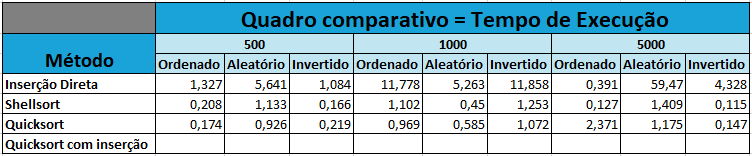
\includegraphics[width=\textwidth]{image3.png}
        \caption[figura 1]{%
            Tabela comparativa de arquivos com até 5000 (cinco mil) entradas%
        }
    \end{figure}
    
    \begin{figure}[h]
        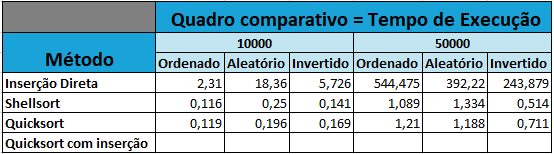
\includegraphics[width=\textwidth]{image4.png}
        \caption[figura 1]{%
            Tabela comparativa de arquivos com 10000 (dez mil) e 50000 (cinquenta mil) entradas%
        }
    \end{figure}

    Com o quadro abaixo providenciado pelos materiais da professora foi possível
    atestar com alguns ajustes de regra de 3, que os métodos Shellsort e
    Quicksort seguem quase que parelhos alguns valores gerados pelo código. Por
    exemplo, multiplicar o N=256 da tabela abaixo por 2, para ter um valor de
    N=512, um valor aproximado do N=500 utilizado em nosso teste.  Optamos por
    esse caminho de comparação porque essa tabela é também em segundos. 

    \begin{figure}[h]
        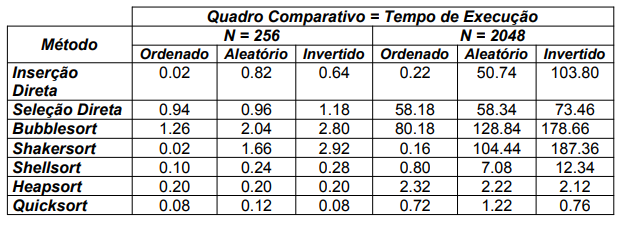
\includegraphics[width=\textwidth]{image5.png}
    \end{figure}

    \fimpagina

    Um outro exemplo, método Shellsort com 500 elementos ordenado em comparação
    com N=256 x 2 da tabela acima também ordenado. No nosso teste dando 0,208
    segundos e no da tabela quando 0,20 segundos.

    A tabela abaixo também foi utilizada na comparação, nos ajudando a entender
    melhor as proporções das medidas de tempo.
            

    \begin{figure}[h]
        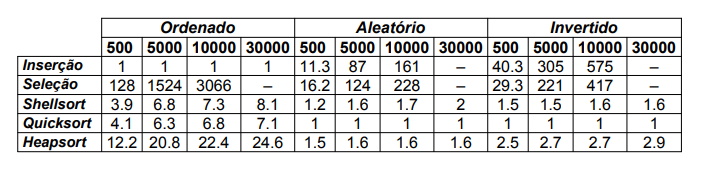
\includegraphics[width=\textwidth]{image2.png}
    \end{figure}

    Os métodos que ficaram com valores muito discrepantes provavelmente se devem
    à diferença de código, por linhas do nosso código, pode ser também por
    diferenças de peça de hardware no que tange memória, processador e todo
    hardware responsável por transferência de dados. Em último caso também pode
    ser porque nós comparamos os CPF’s de um arquivo que pra apenas 1 elemento
    pode possuir mais 3 ou mais 4 informações, atrasando o tempo do método de
    comparação.

    % \fimpagina
    % . . .
    \fimFAESATeX{Desenvolvido com: \vspace*{\baselineskip}}
    \begin{center}
        \href{https://www.github.com/xavier-arthur/faesatex}{\color{blue} Saiba mais clicando aqui}
    \end{center}

\end{document}
